%\documentclass[11pt]{scrartcl}
\documentclass[11pt]{article}
\usepackage[utf8]{inputenc}
\usepackage{cmap}
\usepackage[T1]{fontenc}
\usepackage{lmodern}
\usepackage[brazil]{babel}

%\usepackage{lrsmath}
\usepackage{url}
\usepackage{enumerate}
\usepackage{indentfirst}
\usepackage{acronym}

\usepackage{amsmath}
\usepackage{booktabs}
\usepackage{amssymb}
\usepackage{amsthm}
\usepackage{amscd}
\usepackage{amsfonts}
\usepackage{dsfont}
\usepackage{color}
\usepackage{multicol}
\usepackage{hyperref}

\usepackage[table]{xcolor}

\usepackage{esvect}
\usepackage{graphicx}
\usepackage{float}
\usepackage{indentfirst}
\usepackage{caption}
\usepackage{blkarray}
\newcommand\Mark[1]{\textsuperscript#1}
\usepackage{pgfplots}
\usepackage[english, ruled, linesnumbered]{algorithm2e}
\usepackage{algorithmic}
\usepackage{multirow}
\usepackage{siunitx}
\usepackage{pdflscape}
\usepackage{booktabs}
\usepackage{makecell}
\usepackage{xltabular}
\usepackage{blindtext}
\usepackage{rccol}


\usepackage{graphicx}
\usepackage{tikz}
\usetikzlibrary{arrows,shapes,positioning,shadows,trees}


\tikzset{
  basic/.style  = {draw, text width=2cm, drop shadow, font=\sffamily, rectangle},
  root/.style = {basic, rounded corners=6pt, thin,align=center, fill=green!30,
                   text width=8em},
  level 2/.style = {basic, rounded corners=6pt, thin,align=center, fill=green!30,
                   text width=8em,sibling distance=10mm}
  level 3/.style = {basic, rounded corners=2pt, thin,align=center, fill=green!30,
                    innersep = 10mm,sibling distance=10mm}
}

\usepackage{graphicx}

\usepackage{3dplot}

\newtheorem{defi}{Definição}[section]
\newtheorem{teo}{Teorema}[section]
\newtheorem{cor}{Corolário}[section]
\newtheorem{conj}{Conjectura}[section]
\newtheorem*{propri}{Propriedades}
\newtheorem{pro}{Proposição}[section]
\newtheorem{lema}{Lema}[section]
\newtheorem{obs}{Observação}[section]
\newtheorem{ex}{Exemplo}[section]

\newtheorem*{DGP}{{\emph{Distance Geometry Problem (DGP)}}}

\newtheorem*{iMDGP}{{\emph{interval Molecular Distance Geometry Problem (iMDGP)}}}

\newtheorem*{MDGP}{{\emph{Molecular Distance Geometry Problem (MDGP)}}}

\newtheorem*{DMDGP}{{\emph{Discretizable Molecular Distance Geometry Problem (DMDGP)}}}

\newtheorem*{DDGP}{{\emph{Discretizable Distance Geometry Problem $k =3$ (DDGP$_3$)}}}

\newtheorem*{DVOP}{{\emph{Discretization Vertex Order Problem (DVOP)}}}

\usepackage[top=3cm,bottom=3cm,right=2.5cm,left=2.5cm]{geometry}

\makeatletter
\newcommand{\@chapapp}{}% Not necessary...
\newenvironment{chapquote}[2][2em]
{\setlength{\@tempdima}{#1}%
	\def\chapquote@author{#2}%
	\parshape 1 \@tempdima \dimexpr\textwidth-2\@tempdima\relax%
	\itshape}
{\par\normalfont\hfill--\ \chapquote@author\hspace*{\@tempdima}\par\bigskip}
\makeatother

%\usepackage[backend=biber,style=numeric-comp]{biblatex}
%\usepackage{csquotes}
%\addbibresource{references_bibdesk_papers.bib}

% \usepackage{showlabels} 

\usepackage{geometry}
\geometry{a4paper,top=3cm,left=2.5cm,right=2.5cm}



%\def\Dew{\Delta w}
%\def\Dex{\Delta x}
%\def\Dey{\Delta y}
%\def\Dez{\Delta z}
%\def\Cset{\mathcal{C}}

\begin{document}

%\title{Projeto de Pesquisa}
%\author{Projeto de Atividades Acadêmicas  \\ \textsc{Felipe Delfini Caetano Fidalgo}\thanks{\tt{felipaomat@gmail.com}}}
%\date{Maio de 2015}  
%\thispagestyle{empty}
%
%\maketitle

\begin{titlepage}

\newcommand{\HRule}{\rule{\linewidth}{0.5mm}} % Defines a new command for the horizontal lines, change thickness here

\center % Center everything on the page
 
%----------------------------------------------------------------------------------------
%	HEADING SECTIONS
%----------------------------------------------------------------------------------------

\begin{center}

\includegraphics[scale=0.22]{logoufsc}
\end{center}

\vspace{1cm}

\textsc{\LARGE Universidade Federal de Santa Catarina}\\[0.5cm] % Name of your university/college
{\Large Centro Tecnológico, de Ciências Exatas e Educação \\ Departamento de Matemática}\\[1.5cm] % Major heading such as course name
\textsc{\Large TCC I\\Qualificação\vspace{1.5cm} \\ {Licenciatura em Matemática}}\\[2.0cm] % Minor heading such as course title

%\textsc{\LARGE Universidade Federal de Santa Catarina}\\[0.5cm] % Name of your university/college
%{\Large Centro de Blumenau \\ Departamento de Matemática}\\[1.5cm] % Major heading such as course name
%\textsc{\Large PIBIC \\ Programa Institucional de Bolsas de Iniciação Científica \vspace{1.5cm} \\ {\bf PROJETO DE PESQUISA}}\\[2.0cm] % Minor heading such as course title

%----------------------------------------------------------------------------------------
%	TITLE SECTION
%----------------------------------------------------------------------------------------

\HRule \\[0.4cm]
{ \LARGE \bfseries Introdução à Álgebra Geométrica} \\ [0.4cm] % Title of your document
\HRule \\[2.5cm]
 
%----------------------------------------------------------------------------------------
%	AUTHOR SECTION
%----------------------------------------------------------------------------------------

\begin{minipage}{1\textwidth}
	\begin{center} \large
		Guilherme Philippi (guilherme.philippi@hotmail.com),
		\vspace{0.5cm}
		\\
		\underline{\textsc{Orientador:}} \vspace{0.2cm}
		Felipe Delfini Caetano Fidalgo (felipe.fidalgo@ufsc.br).
	\end{center}
\end{minipage} \\[2cm]


{\large \today} % Date, change the \today to a set date if you want to be precise


\vfill % Fill the rest of the page with whitespace

\end{titlepage}


\begin{abstract}
	A Álgebra Geométrica é uma área relativamente recente da matemática aplicada que proporciona representações algébricas para conceitos geométricos. Convém sua utilização pela sua grande capacidade de unificação, simplificação e generalização de vários objetos matemáticos que possuem interpretação geométrica. Ela integra as noções de vetores, espaços vetoriais, números complexos, quatérnios, tensores e formas diferenciais, proporcionando uma linguagem única para tratar destes conceitos, facilitando a definição e compreensão de problemas. O objetivo principal deste projeto de pesquisa é uma introdução à Álgebra Geométrica, bem como suas aplicações.
\end{abstract}

\tableofcontents

\section{Introdução}

Pode-se dizer que nosso tema de estudo teve início em 1844, com a chamada \textit{Teoria da Expansão} (ou, em alemão, \textit{Ausdehnungslehre} \cite{grassmannLineale}), introduzida por Hermann Günther Grassmann (1809-1877), precursor do que hoje entendemos como a Álgebra Linear. Mas foi somente em 1878 que William Kingdon Clifford (1845-1879) de fato deu à área uma de suas ferramentas fundamentais: o produto geométrico. Na verdade, o termo \textit{Álgebra Geométrica} foi cunhado por Clifford, o que eventualmente fez com que essa área também fosse chamada de Álgebra de Clifford \cite{sommerGeometric}. 
\\


\begin{chapquote}{Clifford, \textit{Applications of Grassmann's Extensive Algebra} \cite{cliffordApplicationsGrassmannAlgebras}}
	``Until recently I was unacquainted with the Ausdehnungsleh, and knew only so much of it as is contained in the author's geometrical papers (...). I may, perhaps, therefore be permitted to express my profound admiration of that extraordinary work, and my conviction that its principles will exercise a vast influence upon the future of mathematical science.''
\end{chapquote}


Existe uma diferença fundamental entre espaço físico e espaço de representação. O espaço físico é onde estão os objetos que estamos interessados em estudar. Já o espaço de representação é tal que proporcione um modelo matemático que abstrai a natureza destes objetos a fim de que possamos manipulá-los. Por exemplo, a Álgebra Linear é um espaço de representação construída a partir do conceito de vetor, isso é, pontos no espaço de representação. A Álgebra Geométrica, no entanto, é um espaço de representação construído sobre o conceito de \textit{subespaços vetoriais}. Para tanto, é necessário que se possa representar os subespaços de forma elementar, como primitivas, assim como são os vetores na Álgebra Linear.

\subsection{O Espaço Multivetorial $\bigwedge\mathbb{R}^n$}

Partiremos de um espaço vetorial. Assim, seja a base $\{e_i\}^n_{i=1}$ para $\mathbb{R}^n$. Um vetor $a$ arbitrário pode ser escrito como a \textit{combinação linear} dos elementos da base, portanto, para $n=3$, $$a = \alpha_1e_1 + \alpha_2e_2 + \alpha_3e_3\in \mathbb{R}^3,$$
em que $\alpha_i\in \mathbb{R}$ é o $i$-ésimo coeficiente de $a$. Podemos interpretar geometricamente $a$ como um segmento de reta orientado, suportado por um subespaço 1-dimensional (uma reta), que passa pela origem de $\mathbb{R}^3$.

\begin{figure}[H]
	\begin{center}
		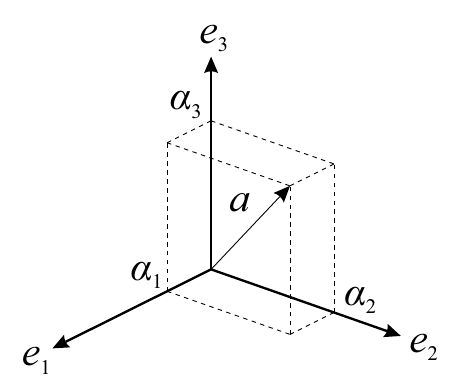
\includegraphics[width=0.25\linewidth]{figures/aR3.png}
	\end{center}
	\caption{Representação do vetor $a$ \cite{leandro2017algebra}}
	\label{fig:r3}
\end{figure}

A Álgebra Exterior de Grassmann trás um novo produto que nos permite operar vetores para construir subespaços de dimensionalidade mais altas. Na Álgebra Geométrica, um subespaço 2-dimensional $C_{\left <2 \right >}$ pode ser expandido como \textbf{produto exterior} de dois vetores $a,b$ linearmente independentes:

$$C_{\left <2 \right >} = a \wedge b,$$
onde o $\wedge$ representa o produto exterior, cujo resultado é um \textit{bivetor} representado como a superfície plana orientada da figura~\ref{fig:2blade}. $a\wedge b$ possui magnitude (representada pela área do disco) e orientação (representada pela seta curva). 

\begin{figure}[H]
	\begin{center}
		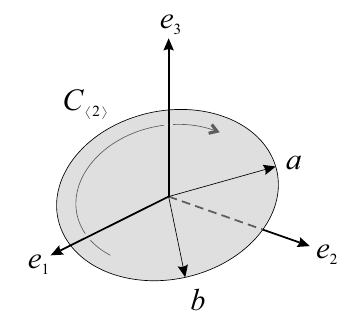
\includegraphics[width=0.25\linewidth]{figures/2blade.png}
	\end{center}
	\caption{Um bivetor $a\wedge b$ representado por um disco apoiado sobre o subespaço 2-dimensional $C_{\left < 2\right >}$, imerso em um espaço tridimensional com base $(e_1,e_2,e_3)$  \cite{leandro2017algebra}.}
	\label{fig:2blade}
\end{figure}

Também pode-se representar um trivetor como o produto exterior de três vetores linearmente independentes $a\wedge b\wedge c$, que expande um subespaço 3-dimensional $D_{\left < 3 \right >}$. A dimensionalidade de $D_{\left < 3 \right >}$ é igual a dimensionalidade do espaço $\mathbb{R}^3$, o que implica que $D_{\left < 3 \right >}$ é uma cópia do volume total, mas agora munido de orientação (representada pela seta em espiral). Isso é, permite-se a construção de pedaços do espaço $\mathbb{R}^3$ com módulo e orientação.

\begin{figure}[H]
	\begin{center}
		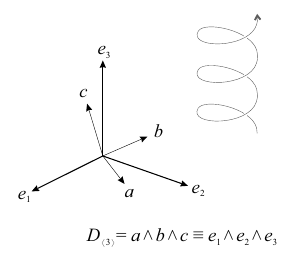
\includegraphics[width=0.3\linewidth]{figures/3blade.png}
	\end{center}
	\caption{Representação do espaço 3-dimensional $D_{\left < 3 \right >}$, expandido pelos vetores $a, b $ e $c$.}
	\label{fig:3blade}
\end{figure}

De modo geral, pode-se expandir subespaços com dimensão $k$ a partir de $k$ vetores li-ne-ar-mente independentes em $\mathbb{R}^n$. Chamamos tais subespaços de \textbf{$k$-blades}, onde $k$ é o \textbf{grau} do blade. Estes serão os elementos primitivos da Álgebra Geométrica. Veja que isso generaliza a Álgebra Vetorial, onde possuíamos apenas os 0-blades e 1-blades, isso é, escalares e vetores. 
\\

Assim, a partir dos elementos do espaço vetorial $\mathbb{R}^n$, podemos construir um \textit{espaço multivetorial} $\bigwedge\mathbb{R}^n$. Isso é, temos $\sum_{k=0}^{n} {n\choose k} = 2^n$ $k$-combinações dos vetores de base de $\mathbb{R}^n$, que descrevem $2^n$ \textbf{blades de base} para $\bigwedge\mathbb{R}^n$. No caso $n =3$, temos

\begin{center}
	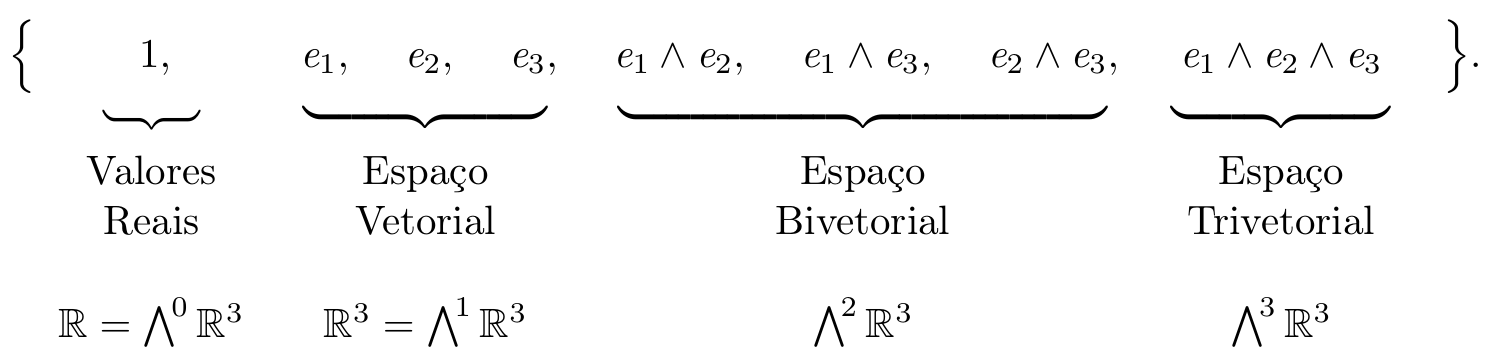
\includegraphics[width=0.75\linewidth]{figures/wr3.png}
\end{center}

A combinação linear destes elementos formam os \textbf{multivetores}. Perceba que há uma simetria entre as dimensões de $\bigwedge^k\mathbb{R}^n$ e $\bigwedge^{n-k}\mathbb{R}^n$.
Por conta de tal simetria, chamamos os elementos de $\bigwedge^{n-1}\mathbb{R}^n$ de \textbf{pseudovetores} e os elementos de $\bigwedge^{n}\mathbb{R}^n$ de \textbf{pseudoescalares}.

Por exemplo, podemos escrever um pseudovetor como 
$$C_{\left < 2\right >} = \alpha_1 e_1\wedge e_2 + \alpha_2 e_1 \wedge e_3 + \alpha_3 e_2 \wedge e_3.$$

\subsection{O Produto Geométrico}

A álgebra exterior definida sobre o espaço multivetorial $\bigwedge\mathbb{R}^3$ é útil para representar o espaço tridimensional, pois contém uma cópia do $\mathbb{R}^3$, o que permite que diversas aplicações geométricas sejam representadas por ela. Porém, como o produto exterior não preserva norma, trabalhar com esta álgebra pode ser um inconveniente para algumas operações (como rotações). Portanto, seria conveniente definir um novo tipo de produto que, dado dois vetores $a$ e $b$, tivéssemos $|\text{``}ab\text{''}| = |a||b|$. Foi o que Clifford fez, e chamou esta nova operação de \textbf{produto geométrico}.
\\

Quando $a,b$ forem números reais (\textit{i.e.}, subespaços 0-dimensionais), o produto geométrico é equivalente a multiplicação de escalares. Quando forem vetores (subespaços 1-dimensionais), esse produto torna-se a soma do produto interno com o produto exterior de Grassmann, isso é, $$ab = a\cdot b + a \wedge b.$$

Assim, através do produto geométrico, podemos operar vetores e obter elementos do espaço multivetorial. Assim, a Álgebra Geométrica pode ser construída a partir de um espaço vetorial $\mathbb{R}^n$ munido do produto geométrico. Esta álgebra também é denotada por $\mathcal C \ell_n$.

\subsection{Modelos de Geometria}

A Álgebra Geométrica também é útil para trabalhar com modelos de geometria diferentes do Euclidiano. Em particular, pretende-se estudar outros dois modelos com diversas aplicações na matemática aplicada, física, engenharia e outras ciências \cite{dorst2010geometric}: O Modelo Homogêneo e o Modelo Conforme.

O Modelo Homogêneo (ou modelo projetivo) possui métrica Euclidiana, com a diferença de que o espaço-base $d$-dimensional está imerso em um espaço de representação com $n = d+1$ dimensões, \textit{i.e.}, possui assinatura $\mathbb{R}^{d+1,0}$. O vetor de base extra é definido como $e_0$ e é interpretado geometricamente como a origem do espaço-base (como representado na Figura~\ref{fig:homogeneo}).

\begin{figure}[H]
	\begin{center}
		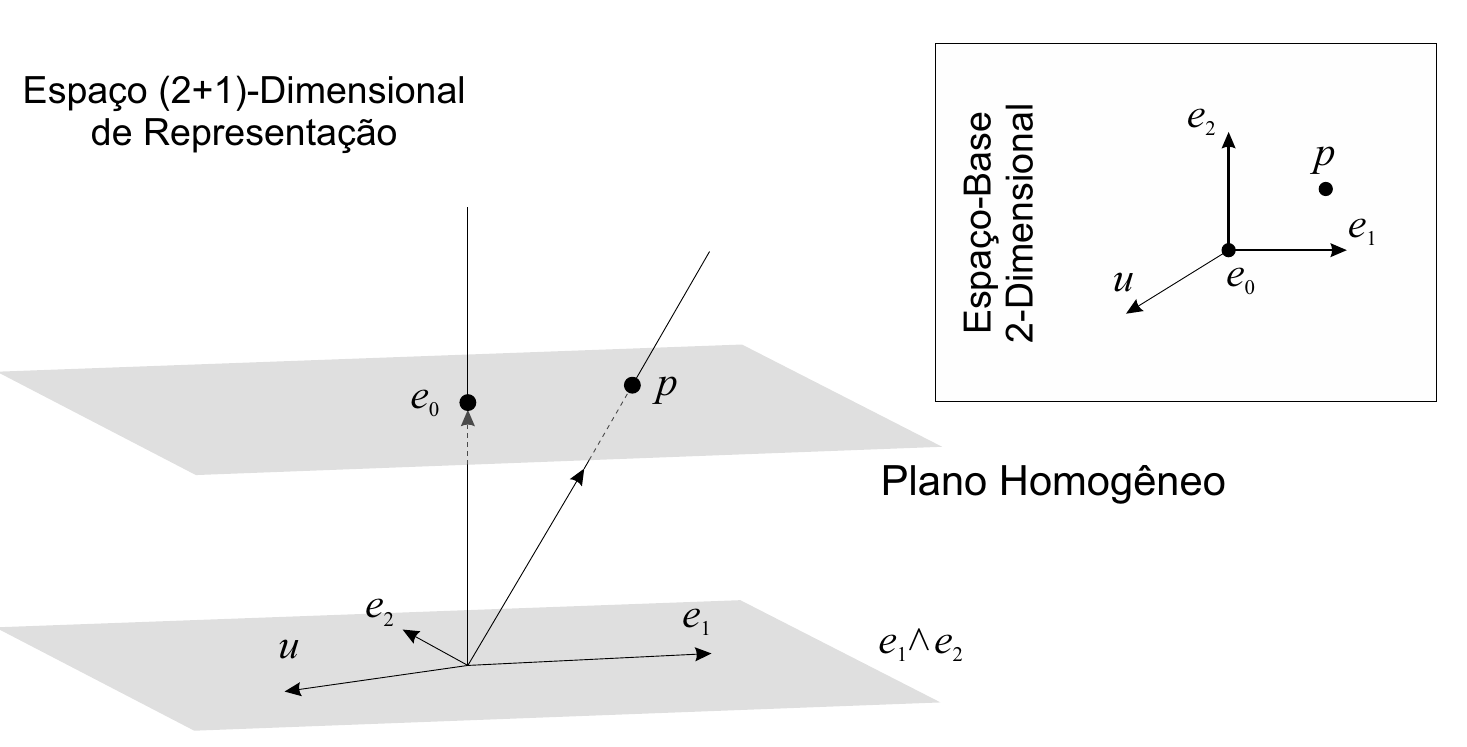
\includegraphics[width=0.75\linewidth]{figures/homogeneo.png}
	\end{center}
	\caption{O plano paralelo a $e_1\wedge e_2$ é a representação homogênea do espaço-base 2-dimensional, exibido como um espaço Cartesiano na imagem em detalhe, à direita \cite{leandro2017algebra}.}
	\label{fig:homogeneo}
\end{figure}

Este modelo é útil para representar translações, pois elas passam a ser transformações lineares. Por conta disso, em Álgebra Linear, quando se trabalha com translações, utilizar o modelo homogêneo permite que se agregue em uma única matriz operações de rotação e translação.
\\

O Modelo Conforme é uma ferramenta que surge quando se deseja trabalhar com transformações de similaridade (que preservam ângulos, paralelismo e razão entre distâncias). Para isso, define-se uma métrica tal que o produto interno entre vetores que codificam \textit{pontos finitos unitários}\footnote{Aqueles descritos como $p =n_0 + \alpha_1e_1 + \dots + \alpha_de_d + \frac{1}{2} \sum_{i=1}^{d}(\alpha_i^2)n_\infty$.} seja diretamente proporcional ao quadrado da distância Euclidiana entre esses pontos. Isso implicaria que o produto interno de um ponto a ele mesmo seria igual nulo.

O Modelo Conforme possui assinatura $\mathbb{R}^{d+1,1}$ e, aqui, as translações também passam a ser lineares. Mais do que isso: elas se tornam transformações ortogonais! Desta maneira, as rotações, reflexões e translações podem ser combinadas em uma única transformação ortogonal, facilitando muito o calculo computacional. As duas dimensões extras são interpretadas geometricamente como o ponto na origem (similar ao Modelo Homogêneo) e o ponto no infinito. 

\begin{figure}[H]
	\begin{center}
		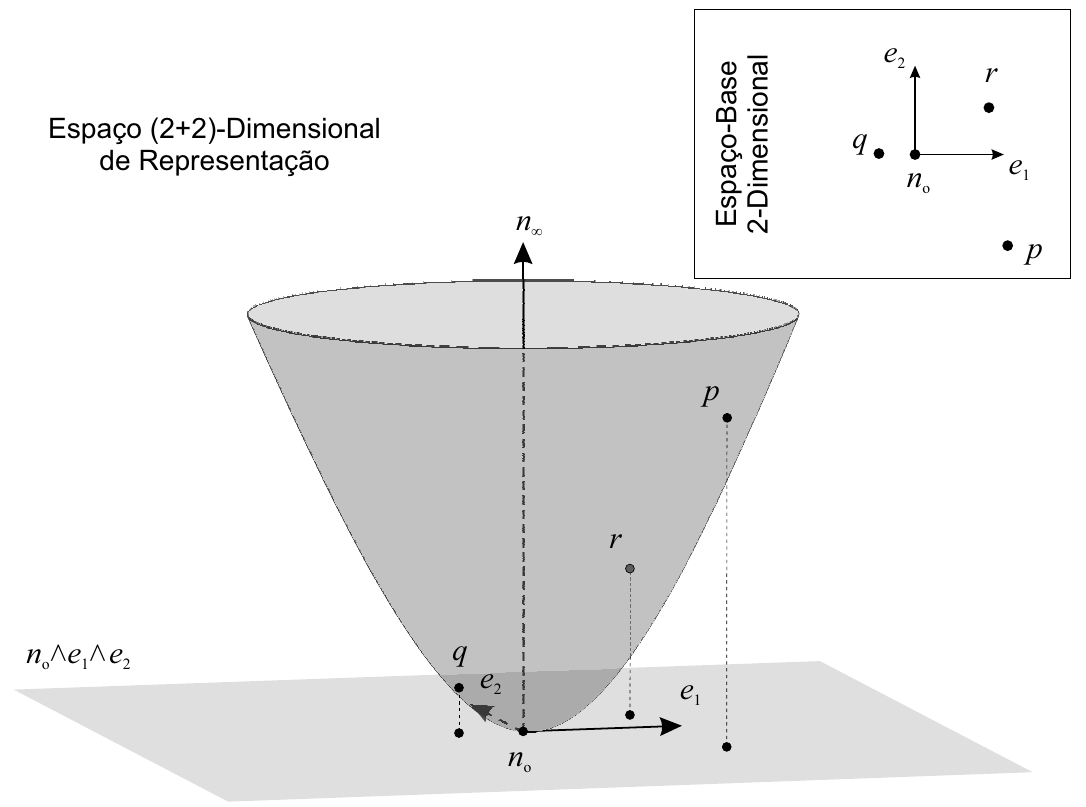
\includegraphics[width=0.75\linewidth]{figures/conforme.png}
	\end{center}
	\caption{O espaço de representação 4-dimensional do modelo conforme, com espaço-base 2-dimensional, é representado graficamente tendo o $n_0$ como dimensão homogênea e ponto na origem do espaço $\{e_1, e_2, e_\infty\}$. Vetores que codificam pontos finitos são representados como pontos no paraboloide \cite{leandro2017algebra}.}
	\label{fig:conforme}
\end{figure}


\section{Objetivos e Justificativa} \label{aims}


\subsection{Objetivo Principal}

O que foi exposto acima torna possível a contextualização do {\bf principal objetivo} deste projeto, que está em estudar a Álgebra Geométrica e seus principais resultados e aplicações. 

\subsection{Objetivos Específicos}

Com o intuito de contemplar isto, ressaltamos alguns dos {\bf objetivos específicos}:

\begin{enumerate}[(1)]

\item Estudar a Álgebra dos subespaços vetoriais com produto interno;

\item Introduzir-se nos espaços métricos;

\item Conhecer o produto exterior, o produto regressivo e o multiespaço vetorial;

\item Estudar o produto escalar de blades e contrações de subespaços vetoriais e suas implicações;

\item Conhecer o produto geométrico e suas implicações, como a Dualidade;

\item Estudar diferentes modelos de geometria, como o Modelo Homogêneo e Modelo Conforme;

\item Estudar como representar os modelos de geometria sob o ponto de vista da Álgebra Geométrica;

\item Estudar as transformações geométricas usando Álgebra Geométrica e suas aplicações.

\end{enumerate}

\section{Metodologia e Resultados Esperados}
 
Inicialmente, pretende-se uma revisão bibliográfica sobre espaços vetoriais e os resultados que interessam ao trabalho. Depois, focar-se-á em uma revisão bibliográfica minuciosa sobre os assuntos elementares da Álgebra Geométrica, utilizando as referências \cite{sommerGeometric}, \cite{leandro2017algebra}, \cite{dorst2010geometric}, \cite{lundholm2009clifford} e \cite{lounestoClifford}, além de artigos e livros citados como referências nestes itens da Literatura. 

Feito isso, algum tempo será dispendido para que o estudante possa confeccionar as seções introdutórias do tema na revisão bibliográfica de seu trabalho de conclusão de curso. Pretende-se um conjunto de definições, resultados e demonstrações dos principais resultados do tema, além de exemplos e discussão para acompanhá-los.
\\

Depois, propõe-se uma ampla revisão bibliográfica para os diferentes modelos de geometria, com foco nos modelos Homogêneo e Conforme e suas caracterizações usando Álgebra Geométrica.

Como antes, espera-se outro intervalo focado na produção das seções referentes ao novo estudo para a revisão bibliográfica do trabalho. Dever-se-á preencher estas seções com exemplos e imagens, a fim de que se possa tomar como intuitiva a manipulação dos conceitos após a leitura.
\\

Por fim, deseja-se estudar a aplicações para a Álgebra Geométrica munidas de tais modelos geométricos. Espera-se que algum estudo prático-computacional possa ser realizado a partir destes conceitos, buscando solucionar problemas descritos através da Álgebra Geométrica.

E, fiel ao método, gastar-se-á algum tempo para escrever sobre as aplicações e as conclusões do estudo, bem como formatá-lo e prepará-lo para submissão. 
\\

Todas as atividades serão acompanhadas de seminários a cada duas semanas para o orientador, a fim de dirimir eventuais dúvidas e traçar planejamentos.

\section{Planos de Trabalho e Cronogramas}

Segue abaixo os planos de trabalho e respectivos cronogramas, ajustados para um semestre de 102 dias (como planejado para o semestre de 2022.2, segundo calendário acadêmico).
	
	\subsection{Plano de Trabalho}
	
	\begin{enumerate}[(1)]
		
	\item \textbf{Levantamento bibliográfico sobre a Álgebra dos subespaços vetoriais com produto interno}
	
	\item \textbf{Demonstrações dos resultados principais}
	
	\item \textbf{Levantamento bibliográfico sobre espaços métricos}
	
	\item \textbf{Preparação de seminários e escrita do trabalho}
	
	\item \textbf{Estudo sobre a Álgebra Exterior, Álgebra Geométrica e suas implicações}
	
	\item \textbf{Demonstrações dos resultados principais}
	
	\item \textbf{Preparação de seminários e escrita do trabalho}
	
	\item \textbf{Levantamento bibliográfico sobre diferentes modelos de geometria, como o Homogêneo e o Conforme}
	
	\item \textbf{Integrar estes modelos à Álgebra Geométrica}
	
	\item \textbf{Demonstrações dos resultados principais}
	
	\item \textbf{Preparação de seminários e escrita do trabalho}
	
	\item \textbf{Estudar aplicações ao que foi estudado}
	
	\item \textbf{Preparação de seminários e escrita do trabalho}
	
	\item \textbf{Finalização do manuscrito e adequação a partir das revisões do orientador}
	
	\end{enumerate}
	
	
	\subsection{Cronograma}
	
\begin{table}[h]
\centering
	\begin{tabular}{| c || c | c | c | c |}
	\hline 
	Atividades & 1$^{\circ}$ mês & 2$^{\circ}$ mês & 3$^{\circ}$ mês & 4$^{\circ}$ mês \\ \hline \hline
	(1) & \cellcolor{gray} &  &  & \\ \hline
	(2) & \cellcolor{gray} &  &  & \\ \hline
	(3) & \cellcolor{gray} &  &  & \\ \hline
	(4) & \cellcolor{gray} &  &  & \\ \hline
	(5) &  & \cellcolor{gray} &  & \\ \hline
	(6) &  & \cellcolor{gray} &  & \\ \hline
	(7) &  & \cellcolor{gray} &  & \\ \hline
	(8) &  &  & \cellcolor{gray} & \\ \hline
	(9) &  &  & \cellcolor{gray} & \\ \hline
	(10) &  &  & \cellcolor{gray} & \\ \hline
	(11) &  &  & \cellcolor{gray} & \\ \hline
	(12) &  &  &  & \cellcolor{gray} \\ \hline
	(13) &  &  &  & \cellcolor{gray} \\ \hline
	(14) &  &  &  & \cellcolor{gray} \\ 
	\hline
	\end{tabular}
\end{table}
	

\phantomsection
\addcontentsline{toc}{section}{Referências}

\bibliographystyle{unsrt}
\bibliography{references}

\end{document}